%% LyX 2.4.0~beta5 created this file.  For more info, see https://www.lyx.org/.
%% Do not edit unless you really know what you are doing.
\documentclass[english,footrule]{foils}
\usepackage[T1]{fontenc}
\usepackage[latin9]{inputenc}
\usepackage{geometry}
\geometry{verbose}
\setcounter{secnumdepth}{1}
\setcounter{tocdepth}{1}
\usepackage{xcolor}
\usepackage{babel}
\usepackage{pifont}
\usepackage{fancybox}
\usepackage{calc}
\usepackage{url}
\usepackage{amsmath}
\usepackage{amsthm}
\usepackage{amssymb}
\usepackage{graphicx}
\usepackage[pdfusetitle,
 bookmarks=true,bookmarksnumbered=false,bookmarksopen=false,
 breaklinks=false,pdfborder={0 0 1},backref=false,colorlinks=false]
 {hyperref}

\makeatletter

%%%%%%%%%%%%%%%%%%%%%%%%%%%%%% LyX specific LaTeX commands.
\newcommand{\noun}[1]{\textsc{#1}}

%%%%%%%%%%%%%%%%%%%%%%%%%%%%%% Textclass specific LaTeX commands.
\theoremstyle{definition}
\newtheorem{defn}{\protect\definitionname}

%%%%%%%%%%%%%%%%%%%%%%%%%%%%%% User specified LaTeX commands.
\usepackage{graphicx,xcolor}
% darker colors for better slides...
\definecolor{green}{RGB}{0, 180, 0}
\definecolor{cyan}{RGB}{0, 180, 180}
\definecolor{yellow}{RGB}{211,211,0}

%\usepackage{xcolor}
\renewcommand{\labelitemi}{$\textcolor{blue}{\bullet}$}
\renewcommand{\labelitemii}{$\textcolor{teal}{\Rightarrow}$}
\renewcommand{\labelitemiii}{$\textcolor{red}{\rightarrow}$}
\renewcommand{\labelitemiv}{$\textcolor{brown}{\circ}$}

\newcommand{\T}{\mathrm{T}}  % transpose
\newcommand{\PP}{\mathrm{P}}  % probability
\newcommand{\dd}{\mathrm{d}} % integration dx
\newcommand{\ee}{\mathrm{e}} % exponential
\newcommand{\E}{\mathrm{E}} % expectation


% DA
\newcommand{\xf}{\mathbf{x}^{\mathrm{f}}}
\newcommand{\xa}{\mathbf{x}^{\mathrm{a}}}
\newcommand{\xb}{\mathbf{x}^{\mathrm{b}}}
\newcommand{\xt}{\mathbf{x}^{\mathrm{t}}}
\newcommand{\barx}{\overline{\mathbf{x}}}

\newcommand{\x}{\mathbf{x}}
\newcommand{\y}{\mathbf{y}}
\newcommand{\yo}{\mathbf{y}^{\mathrm{o}}}
\newcommand{\bary}{\overline{\mathbf{y}}}

%\newcommand{\X}{\mathbf{X}}
\newcommand{\Xf}{\mathbf{X}_{\mathrm{f}}}
\newcommand{\Xa}{\mathbf{X}_{\mathrm{a}}}

%\newcommand{\bY}{\mathbf{Y}}
\newcommand{\Yf}{\mathbf{Y}_{\mathrm{f}}}

\newcommand{\w}{\mathbf{w}}
%\newcommand{\W}{\mathbf{W}}

\newcommand{\z}{\mathbf{z}}
\newcommand{\dv}{\mathbf{d}}

%\newcommand{\Pa}{\mathbf{P}^{\mathrm{a}}}
\newcommand{\Pf}{\mathbf{P}^{\mathrm{f}}}

%\newcommand{\K}{\mathbf{K}}
%\newcommand{\B}{\mathbf{B}}
\newcommand{\R}{\mathbf{R}}
\newcommand{\Q}{\mathbf{Q}}
%\newcommand{\Ho}{\mathbf{H}}
\newcommand{\Hc}{\mathcal{H}}

%\newcommand{\M}{\mathbf{M}}
\newcommand{\Mc}{\mathcal{M}}
\newcommand{\Mk}{\mathbf{M}_{k}}
\newcommand{\Mkk}{\mathbf{M}_{k+1}}

\newcommand{\Rn}{\mathbb{R}^{n}}
\newcommand{\Rp}{\mathbb{R}^{p}}
\newcommand{\Rm}{\mathbb{R}^{m}}
\newcommand{\Rnn}{\mathbb{R}^{n\times n}}
\newcommand{\Rpp}{\mathbb{R}^{p\times p}}
\newcommand{\Id}{\mathbf{I}}

\newcommand{\ea}{\boldsymbol{\epsilon}^{\mathrm{a}}}
\newcommand{\eb}{\boldsymbol{\epsilon}^{\mathrm{b}}}
\newcommand{\ef}{\boldsymbol{\epsilon}^{\mathrm{f}}}
\newcommand{\eo}{\boldsymbol{\epsilon}^{\mathrm{o}}}
\newcommand{\eq}{\boldsymbol{\epsilon}^{\mathrm{q}}}

\newcommand{\zero}{\mathbf{0}}
\newcommand{\one}{\mathbf{1}}
\newcommand{\onehalf}{\frac{1}{2}}


\newcommand{\nn}{\nonumber\\}
\newcommand{\tr}{\rm Tr}
\def\({\left(}
\def\){\right)}

%\newcommand{\bu}{\mathbf{u}}
\newcommand{\baru}{\overline{\mathbf{u}}}
\newcommand{\bh}{\mathbf{h}}
\newcommand{\bv}{\mathbf{v}}
\newcommand{\bz}{\mathbf{z}}

%\newcommand{\bP}{\mathbf{P}}
\newcommand{\bS}{\mathbf{S}}
%\newcommand{\bA}{\mathbf{A}}
\newcommand{\bV}{\mathbf{V}}
\newcommand{\bT}{\mathbf{T}}
%\newcommand{\bU}{\mathbf{U}}
\newcommand{\bE}{\mathbf{E}}
\newcommand{\bZ}{\mathbf{Z}}
\newcommand{\bC}{\mathbf{C}}
\newcommand{\bL}{\mathbf{L}}

\newcommand{\bOmega}{\mathbf{\Omega}}
\newcommand{\bLambda}{\mathbf{\Lambda}}
\newcommand{\bdelta}{\bm{\delta}}
\newcommand{\brho}{\boldsymbol{\rho}}
\newcommand{\beps}{\boldsymbol{\epsilon}}
\newcommand{\bSigma}{\mathbf{\Sigma}}
\newcommand{\balpha}{\boldsymbol{\alpha}}
%\newcommand{\bbeta}{\bm{\beta}}
%\newcommand{\btheta}{\bm{\theta}}
\newcommand{\ceta}{\boldsymbol{\eta}}

%%MB
\newcommand{\Hess}{\mathrm{H}}
\newcommand{\Tc}{\mathcal{T}}

%%MA
%\newcommand{\dd}{\mathrm{d}}
\newcommand{\Pb}{\mathbf{P}^{\mathrm{b}}}

\makeatother

\providecommand{\definitionname}{Definition}

\begin{document}
\title{Data Assimilation\\
\rule[0.5ex]{1\columnwidth}{3pt}}
\author{Mark Asch - CSU/IMU/2023}
\date{\bigskip{}
\bigskip{}
\bigskip{}
\noun{\includegraphics[scale=1.2]{graphics/3D4D-Var}}}
\maketitle

\MyLogo{Data Assim. Intro - M. Asch - Lecture 01}

\foilhead{Outline of the course (I)}

\textcolor{blue}{Adjoint methods and variational data assimilation
(4h)}
\begin{enumerate}
\item \textcolor{red}{Introduction to data assimilation: setting, history,
overview, definitions.}
\item \textcolor{lightgray}{Optimization methods.}
\item \textcolor{lightgray}{Adjoint method.}
\item \textcolor{lightgray}{Variational data assimilation methods: }
\begin{enumerate}
\item \textcolor{lightgray}{3D-Var, }
\item \textcolor{lightgray}{4D-Var.}
\end{enumerate}
\end{enumerate}

\foilhead{Outline of the course (II)}

\textcolor{blue}{Statistical estimation, Kalman filters and sequential
data assimilation (4h)}
\begin{enumerate}
\item \textcolor{lightgray}{Introduction to statistical DA.
\item Statistical estimation.
\item The Kalman filter.
\item Nonlinear extensions and ensemble filters.}
\end{enumerate}

\foilhead{Reference Textbooks}
\begin{center}
\includegraphics[width=0.8\textwidth]{graphics/FA11_Asch-Boucquet_cover10-24-16}
\par\end{center}

\begin{center}
\includegraphics[width=0.8\textwidth]{graphics/MN06_ASCH_COVER_B_V6}
\par\end{center}

\foilhead{$\;$}

\vfill{}

\begin{center}
{\Large\textbf{\textcolor{blue}{INTRODUCTION}}}{\Large\par}
\par\end{center}

\vfill{}


\foilhead{\textcolor{blue}{What is data assimilation?}}
\begin{itemize}
\item Simplest view: a method of combining observations with model output. 
\item Why do we need data assimilation? Why not just use the observations?
(cf. \textcolor{green}{Regression})
\begin{itemize}
\item We want to predict the future! 

\begin{itemize}
\item For that we need models. 
\item But when models are not constrained periodically by reality, they
are of little value. 
\item Therefore, it is necessary to \textcolor{magenta}{fit the model state
as closely as possible to the observations}, before a prediction is
made.
\end{itemize}
\end{itemize}
\end{itemize}
\begin{defn}
Data assimilation (DA) is the approximation of the true state of some
physical system at a given time, by combining time-distributed observations
with a dynamic model in an optimal way.
\end{defn}

\foilhead{\textcolor{blue}{Data assimilation methods}}

There are two major classes of methods: 
\begin{enumerate}
\item \textcolor{magenta}{Variational methods} where we explicitly minimize
a cost function using optimization methods.
\item \textcolor{magenta}{Statistical methods} where we compute the best
linear unbiased estimate (BLUE) by algebraic computations using the
Kalman filter.
\end{enumerate}
\begin{itemize}
\item They provide the same result in the linear case, which is the only
context where their optimality can be rigorously proved. 
\item They both have difficulties in dealing with non-linearities and large
problems. 
\item The error statistics that are required by both, are in general poorly
known.
\end{itemize}

\foilhead{\textcolor{blue}{Introduction: approaches}}
\begin{itemize}
\item DA is an approach for solving a specific class of \textcolor{magenta}{inverse},
or parameter estimation problems, where the parameter we seek is the
\textcolor{magenta}{initial condition}.
\item Assimilation problems can be approached from many directions (depending
on your background/preferences):

\begin{itemize}
\item \textcolor{blue}{control theory};
\item \textcolor{blue}{variational calculus;}
\item \textcolor{magenta}{statistical estimation theory;}
\item \textcolor{magenta}{probability theory,}
\item stochastic differential equations.
\end{itemize}
\item Newer approaches (see \textcolor{magenta}{Advanced} Course): nudging
methods, reduced methods, ensemble methods and hybrid methods that
combine variational and statistical approaches, \textcolor{magenta}{Machine/Deep
Learning based approaches}.
\end{itemize}

\foilhead{\textcolor{blue}{Introduction: applications}}
\begin{enumerate}
\item Navigation: important application of the Kalman filter.
\item Remote sensing: satellite data.
\item Geophysics: seismic exploration, geo-prospection, earthquake prediction.
\item Air and noise pollution, source estimation
\item Weather forecasting.
\item Climatology. Global warming.
\item Epidemiology.
\item Forest fire evolution.
\item Finance.
\end{enumerate}

\foilhead{\textcolor{blue}{Introduction: nonlinearity...}}

The problems of data assimilation (in particular) and inverse problems
in general arise from:
\begin{enumerate}
\item The \textcolor{magenta}{nonlinear dynamics }of the physical model
equations.
\item The nonlinearity of the \textcolor{magenta}{inverse problem}.
\end{enumerate}

\foilhead{\textcolor{blue}{Introduction: iterative process...}}
\begin{center}
\includegraphics[width=1.05\textwidth]{graphics/model-assimilation-observations}
\par\end{center}
\begin{itemize}
\item Closely related to (see Advanced Course)
\begin{itemize}
\item the\textcolor{magenta}{{} inference cycle }
\item \textcolor{magenta}{machine learning}...
\end{itemize}
\end{itemize}

\foilhead{$\;$}

\vfill{}

\begin{center}
{\Large\textbf{\textcolor{blue}{FORWARD AND INVERSE PROBLEMS}}}{\Large\par}
\par\end{center}

\vfill{}


\foilhead[-0.5in]{\textcolor{blue}{Forward and Inverse problems}}
\begin{center}
\includegraphics[width=1\textwidth]{graphics/direct_inverse}
\par\end{center}
\begin{itemize}
\item Consider a parameter-dependent dynamical system,
\[
\frac{dz}{dt}=g(t,z;\theta),\qquad z(t_{0})=z_{0},
\]
 with $g$ known, $\theta\in\Theta,$ $z(t)\in\mathbb{R}^{k}.$
\end{itemize}
\begin{description}
\item [{Forward:}] \textcolor{blue}{Given $\theta,$} \textcolor{blue}{$z_{0},$
}\textcolor{orange}{find $z(t)$} for $t\ge t_{0}.$
\item [{Inverse:}] \textcolor{orange}{Given $z(t)$}\textcolor{green}{{}
}for $t\ge t_{0},$ \textcolor{blue}{find $\theta\in\Theta.$}
\end{description}

\foilhead{\textcolor{blue}{Observations}}
\begin{itemize}
\item Observation \textcolor{magenta}{equation}:
\[
f(t,\theta)=\mathcal{H}z(t,\theta),
\]
where $\mathcal{H}$ is the observation operator\textemdash to account
for the fact that observations are never completely known (in space-time). 
\item Usually we have a finite number of discrete (space-time) \textcolor{magenta}{observations}
\[
\left\{ \tilde{y}_{j}\right\} _{j=1}^{n},
\]
where 
\[
\tilde{y}_{j}\approx f(t_{j},\theta).
\]
\end{itemize}

\foilhead{\textcolor{blue}{Model-driven and data-driven inverse problems}}
\begin{itemize}
\item \textcolor{magenta}{Model}-driven:
\[
\tilde{y}_{j}=f(t_{j},\theta)
\]
\item \textcolor{magenta}{Data}-driven:
\[
\tilde{y}_{j}=f(t_{j},\theta)+\varepsilon_{j},
\]
where $\varepsilon_{j}$ is error and requires that we introduce \textcolor{magenta}{variability/uncertainty}
into the modeling and analysis.
\end{itemize}

\foilhead{\textcolor{blue}{Well-posedness}}
\begin{enumerate}
\item \textcolor{magenta}{Existence}
\item \textcolor{magenta}{Uniqueness}
\item \textcolor{magenta}{Continuous dependence} of solutions on observations.
\end{enumerate}
\begin{dinglist}{52}
\item The existence and uniqueness together are also known as \textcolor{red}{``identifiability''}.
\item The continuous dependence is related to the \textcolor{red}{``stability''}
of the inverse problem.
\end{dinglist}

\foilhead{\textcolor{blue}{Well-posedness (mathematical)}}
\begin{defn}
Let $X$ and $Y$ be two normed spaces and let $K\::\:X\rightarrow Y$
be a linear or nonlinear map between the two. The problem of finding
$x$ given $y$ such that 
\[
Kx=y
\]
is well-posed if the following three properties hold:
\end{defn}
\begin{description}
\item [{WP1}] Existence\textemdash for every $y\in Y$ there is (at least)
one solution $x\in X$ such that $Kx=y.$ 
\item [{WP2}] Uniqueness\textemdash for every $y\in Y$ there is at most
one $x\in X$ such that $Kx=y.$ 
\item [{WP3}] Stability\textemdash the solution $x$ depends continuously
on the data $y$ in that for every sequence $\left\{ x_{n}\right\} \subset X$
with $Kx_{n}\rightarrow Kx$ as $n\rightarrow\infty,$ we have that
$x_{n}\rightarrow x$ as $n\rightarrow\infty.$ 
\end{description}
\begin{itemize}
\item This concept of ill-posedness will help us to understand and distinguish
between direct and inverse models. 
\item It will provide us with basic comprehension of the methods and algorithms
that will be used to solve inverse problems. 
\item Finally, it will assist us in the analysis of ``what went wrong?''
when we attempt to solve the inverse problems.
\end{itemize}

\foilhead{\textcolor{blue}{Ill-posedness of inverse problems}}
\begin{center}
\noindent\shadowbox{\begin{minipage}[t]{1\columnwidth - 2\fboxsep - 2\fboxrule - \shadowsize}%
\begin{center}
\textcolor{red}{All inverse problems are notoriously ill-posed!!!}
\par\end{center}%
\end{minipage}}
\par\end{center}

Simplest case: one observation $\tilde{y}$ for $f(\theta)$ and we
need to find the pre-image
\[
\theta^{*}=f^{-1}(\tilde{y})
\]
for a given $\tilde{y}.$ 

\begin{center}
\includegraphics[scale=0.6]{\string"/Users/markasch/Dropbox/3Teaching/Assim/Assim_2012_CIMPA _ Caracas/graphics/preimage\string".pdf}
\par\end{center}

\foilhead{\textcolor{blue}{Simplest case}}
\begin{center}
\includegraphics[scale=0.6]{\string"/Users/markasch/Dropbox/3Teaching/Assim/Assim_2012_CIMPA _ Caracas/graphics/illposedex\string".pdf}
\par\end{center}
\begin{dinglist}{56}
\item \textcolor{magenta}{Non-existence}: there is no $\theta_{3}$ such
that $f(\theta_{3})=y_{3}$
\item \textcolor{magenta}{Non-uniqueness}: $y_{j}=f(\theta_{j})=f(\widetilde{\theta}_{j})$
for $j=1,2.$ 
\item \textcolor{magenta}{Lack of continuity }of inverse map: $\left|y_{1}-y_{2}\right|$
small $\nRightarrow$ $\left|f^{-1}(y_{1})-f^{-1}(y_{2})\right|=\left|\theta_{1}-\tilde{\theta}_{2}\right|$
small.
\end{dinglist}

\foilhead{\textcolor{blue}{Why is this so important???}}

Couldn't we just apply a good \textcolor{magenta}{least squares} algorithm
(for example) to find the best possible solution?
\begin{itemize}
\item Define $J(\theta)=\left|y_{1}-f(\theta)\right|^{2}$ for a given $y_{1}$
\item Apply a standard iterative scheme, such as direct search or gradient-based
\textcolor{magenta}{minimization}, to obtain a solution
\item Newton's method:
\[
\theta^{k+1}=\theta^{k}-\left[J'(\theta^{k})\right]^{-1}J(\theta^{k})
\]
\end{itemize}

\foilhead{\textcolor{blue}{Newton iterations}}
\begin{center}
\includegraphics[scale=0.6]{\string"/Users/markasch/Dropbox/3Teaching/Assim/Assim_2012_CIMPA _ Caracas/graphics/newton\string".pdf}
\par\end{center}
\begin{itemize}
\item $\theta^{k+1}=\theta^{k}-\left[J'(\theta^{k})\right]^{-1}J(\theta^{k}),$
$J(\theta)=\left|y_{1}-f(\theta)\right|^{2}$ 
\item $J'(\theta)=2\left(y_{1}-f(\theta)\right)\left(-f'(\theta)\right)$ 
\end{itemize}
\begin{dinglist}{56}
\item $J'(\theta^{0})=2(-)(--)<0\quad\Rightarrow\quad\theta^{1}>\theta^{0},$
etc.
\item $J'(\tilde{\theta}^{0})=2(-)(-+)>0\quad\Rightarrow\quad\widetilde{\theta}^{1}<\tilde{\theta}^{0},$
etc.
\end{dinglist}

\foilhead{\textcolor{blue}{What went wrong?}}
\begin{dinglist}{56}
\item This behavior is not the fault of steepest descent algorithms.
\item It is a manifestation of the\textcolor{magenta}{{} inherent ill-posedness}
of the problem.
\item How to fix this problem is the subject of much research over the past
\textcolor{red}{50 years}!!!
\end{dinglist}
\begin{dinglist}{52}
\item Many remedies (fortunately) exist....

\begin{dinglist}{52}
\item explicit and implicit constrained optimizations
\item regularization and penalization
\item \textcolor{magenta}{machine learning}...
\end{dinglist}
\end{dinglist}

\foilhead{\textcolor{blue}{Example: Tikhonov regularization}}
\begin{description}
\item [{Idea}] is to replace the ill-posed problem for $J(\theta)=\left|y_{1}-f(\theta)\right|^{2}$
by a ``nearby'' problem for
\[
J_{\beta}(\theta)=\left|y_{1}-f(\theta)\right|^{2}+\beta\left|\theta-\theta_{0}\right|^{2}
\]
where $\beta$ is ``suitably chosen'' regularization/penalization
parameter\textemdash see below for details.
\end{description}
\begin{dinglist}{52}
\item When it is done correctly, TR provides convexity and compactness.
\end{dinglist}
\begin{dinglist}{56}
\item Even when done correctly, it \textcolor{red}{\emph{modifies the problem}}
and new solutions may be far from the original ones.
\item It is not trivial to regularize correctly or even to know if you have
succeeded...
\end{dinglist}

\foilhead{\textcolor{blue}{Examples of ill-posedness}}

We illustrate these with 2 numerical examples.
\begin{dinglist}{52}
\item Duffing's equation.
\item Estimation of seismic travel time.
\end{dinglist}

\foilhead{\textcolor{blue}{Nonlinearity: Duffing}}

The highly \textcolor{blue}{nonlinear Duffing's equation},
\[
\ddot{x}+0.05\dot{x}+x^{3}=7.5\cos t
\]
exhibits great \textcolor{blue}{sensitivity to the initial conditions}.
We can observe that two very closely spaced initial states lead to
a large discrepancy in the trajectories.
\begin{itemize}
\item let $x(0)=3$ and $\dot{x}(0)=4$ be the true initial state;
\item introduce an error of $0.03$\% - here we have an accurate forecast
until $t=35$;
\item introduce an error of $0.06$\% - - here we only have an accurate
forecast until $t=20.$
\end{itemize}
\begin{center}
\includegraphics[width=0.45\paperheight]{\string"/Users/markasch/Dropbox/3Teaching/Assim/Assim_2012_CIMPA _ Caracas/matlab/perturb03\string".pdf}
\par\end{center}

\begin{center}
\includegraphics[width=0.45\paperheight]{\string"/Users/markasch/Dropbox/3Teaching/Assim/Assim_2012_CIMPA _ Caracas/matlab/perturb06\string".pdf}
\par\end{center}

\foilhead[-0.5in]{\textcolor{blue}{Non uniqueness: seismic travel-time tomography}}
\begin{center}
\includegraphics[scale=0.7]{\string"/Users/markasch/Dropbox/3Teaching/Assim/Assim_2012_CIMPA _ Caracas/graphics/travel\string".png}
\par\end{center}

A signal seismic ray passes through a 2-parameter block model.
\begin{itemize}
\item \textcolor{blue}{unknowns} are the 2 block slownesses (inverse of
seismic velocity) $\left(\Delta s_{1},\Delta s_{2}\right)$
\item \textcolor{blue}{data} is the observed travel time of the ray, $\Delta t_{1}$
\item \textcolor{blue}{model} is the linearized travel time equation,
\[
\Delta t_{1}=l_{1}\Delta s_{1}+l_{2}\Delta s_{2}
\]
where $l_{j}$ is the length of the ray in the $j$-th block.
\end{itemize}
Clearly we have \textcolor{magenta}{one equation} for \textcolor{magenta}{two
unknowns} and hence there is \textcolor{red}{no unique solution}.

\foilhead{\textcolor{blue}{Inverse Problems: General Formulation}}
\begin{itemize}
\item All inverse problems share a \textcolor{magenta}{common formulation}. 
\item Let the \textcolor{magenta}{model parameters}\footnote{Applied mathematicians often call the equation $G(m)=d$ a mathematical
model and $m$ the parameters. Other scientists call $G$ the forward
operator and $m$ the model. We will adopt the more mathematical convention,
where $m$ will be referred to as the model parameters, $G$ the model
and $d$ the data.} be a vector (in general, a multivariate random variable), $\mathbf{m},$
and the \textcolor{magenta}{data} be $\mathbf{d},$
\begin{align*}
\mathbf{m} & =\left(m_{1},\ldots,m_{p}\right)\in\mathcal{M},\\
\mathbf{d} & =\left(d_{1},\ldots,d_{n}\right)\in\mathcal{D},
\end{align*}
where 
\begin{itemize}
\item $\mathcal{M}$ and $\mathcal{D}$ are the corresponding model parameter
space and data space. 
\end{itemize}
\item The mapping $G\colon\mathcal{M}\rightarrow\mathcal{D}$ is defined
by the\textcolor{magenta}{{} direct }(or forward) model 
\begin{equation}
\mathbf{d}=g(\mathbf{m}),\label{eq:det-inv-pb}
\end{equation}
where
\begin{itemize}
\item $g\in G$ is an operator that describes the ``physical'' model and
can take numerous forms, such as algebraic equations, differential
equations, integral equations, or linear systems. 
\end{itemize}
\item Then we can add the \textcolor{magenta}{observations }or predictions,
$\mathbf{y}=(y_{1},\ldots,y_{r}),$ corresponding to the mapping from
data space into observation space, $H\colon\mathcal{D}\rightarrow\mathcal{Y},$
and described by 
\[
\mathbf{y}=h(\mathbf{d})=h\left(g(\mathbf{m})\right),
\]
where
\begin{itemize}
\item $h\in H$ is the \textcolor{magenta}{observation operator}, usually
some projection into an observable subset of $\mathcal{D}.$ 
\end{itemize}
\item Note that, in addition, there will be some \textcolor{magenta}{random
noise} in the system, usually modeled as additive noise, giving the
more realistic, stochastic direct model 
\begin{equation}
\mathbf{d}=g(\mathbf{m})+\mathbf{\epsilon},\label{eq:stat-inv-pb}
\end{equation}
where
\begin{itemize}
\item $\mathbf{\epsilon}$ is a random vector.
\end{itemize}
\end{itemize}

\foilhead{\textcolor{blue}{Inverse Problems: Classification}}
\begin{itemize}
\item We can now classify inverse problems as:
\begin{itemize}
\item \textcolor{magenta}{deterministic} inverse problems that solve (\ref{eq:det-inv-pb})
for $\mathbf{m},$ 
\item \textcolor{magenta}{statistical} inverse problems that solve (\ref{eq:stat-inv-pb})
for $\mathbf{m}.$ 
\end{itemize}
\item The first class will be treated by linear algebra and \textcolor{magenta}{optimization
}methods. 
\item The latter can be treated by a \textcolor{magenta}{Bayesian (filtering)
}approach, and by weighted least-squares, maximum likelihood and DA
techniques 
\item Both classes can be further broken down into:
\begin{itemize}
\item \textcolor{magenta}{Linear }inverse problems, where (\ref{eq:det-inv-pb})
or (\ref{eq:stat-inv-pb}) are linear equations. These include linear
systems\textemdash that are often the result of discretizing (partial)
differential equations\textemdash and integral equations. 
\item \textcolor{magenta}{Nonlinear} inverse problems where the algebraic
or differential operators are nonlinear. 
\end{itemize}
\item Finally, since most inverse problems cannot be solved explicitly,
\textcolor{magenta}{computational methods} are indispensable for their
solution\textemdash see {[}Asch2022{]} 
\item . Also note that we will be inverting here between the model and data
spaces, that are usually both of high dimension and thus this model-based
inversion will invariably be \textcolor{magenta}{computationally expensive}.
\item This will motivate us to employ 
\begin{itemize}
\item \textcolor{magenta}{reduced order methods} based on suitable projections, 
\item inversion between the data and observation spaces in a purely data-driven
approach, using \textcolor{magenta}{machine learning methods} (see
Advanced Course)
\end{itemize}
\end{itemize}

\foilhead[-0.5in]{\textcolor{blue}{Tikhonov Regularization: Introduction}}
\begin{itemize}
\item Tikhonov regularization (TR) is probably the most widely used method
for\textcolor{magenta}{{} regularizing} ill-posed, discrete and continuous
\textcolor{magenta}{inverse problems}. 
\item Note that the \textcolor{magenta}{LASSO} and \textcolor{magenta}{ridge
regression} methods\textemdash see ML Lectures\textemdash are special
cases of TR,
\item The theory is the subject of entire books...
\item Recall:
\begin{itemize}
\item the objective of TR is to reduce, or remove, ill-posedness in optimization
problems by modifying the objective function. 
\item the three sources of ill-posedness: non-existence, non-uniqueness
and sensitivity to perturbations. 
\item TR, in principle, addresses and alleviates \textcolor{magenta}{all
three sources} of ill-posedness and is thus a vital tool for the solution
of inverse problems. 
\end{itemize}
\end{itemize}

\foilhead{\textcolor{blue}{Tikhonov Regularization: Formulation}}
\begin{itemize}
\item The most general TR \textcolor{magenta}{objective function} is 
\[
\mathcal{T}_{\alpha}(\mathbf{m};\mathbf{d})=\rho\left(G(\mathbf{m}),\mathbf{d}\right)+\alpha J(\mathbf{m}),
\]
where
\begin{itemize}
\item $\rho$ is the \textcolor{magenta}{\emph{data discrepancy functional}}
that quantifies the difference between the model output and the measured
data; 
\item $J$ is the \textcolor{magenta}{\emph{regularization functional}}
that represents some desired quality of the sought for model parameters,
usually smoothness; 
\item $\alpha$ is the \emph{r}\textcolor{magenta}{\emph{egularization parameter}}
that needs to be \textcolor{magenta}{\emph{tuned}}, and determines
the relative importance of the regularization term. 
\end{itemize}
\item Each domain, each application and each context will require \textcolor{magenta}{\emph{specific
choices }}of these three items, and often we will have to rely either
on previous experience, or on some sort of numerical experimentation
(trial-and-error) to make a good choice. 
\item In some cases there exist empirical algorithms, in particular for
the choice of $\alpha.$
\end{itemize}

\foilhead{\textcolor{blue}{Tikhonov Regularization: Discrepancy}}

The most common \textcolor{magenta}{\emph{discrepancy functions}}
are:\index{Tikhonov regularization (TR)!discrepancy functions} 
\begin{itemize}
\item \textcolor{magenta}{\emph{least-squares}}, 
\[
\rho_{\mathrm{LS}}(\mathbf{d}_{1},\mathbf{d}_{2})=\frac{1}{2}\Vert\mathbf{d}_{1}-\mathbf{d}_{2}\Vert_{2}^{2},
\]
\item \textcolor{magenta}{\emph{1-norm}}, 
\[
\rho_{1}(\mathbf{d}_{1},\mathbf{d}_{2})=\vert\mathbf{d}_{1}-\mathbf{d}_{2}\vert,
\]
\item \textcolor{magenta}{\emph{Kullback-Leibler distance}},\index{Kullback-Leibler distance}
\[
\rho_{\mathrm{KL}}(d_{1},d_{2})=\left\langle d_{1},\log(d_{1}/d_{2})\right\rangle ,
\]
where $d_{1}$ and $d_{2}$ are considered here as probability density
functions. This discrepancy is valid in the Bayesian context.
\end{itemize}

\foilhead[-0.5in]{\textcolor{blue}{Tikhonov Regularization: Regularization}}

The most common \textcolor{magenta}{\emph{regularization functionals}}\index{Tikhonov regularization (TR)!regularization functionals}
are derivatives of order one or two.
\begin{itemize}
\item \textcolor{magenta}{\emph{Gradient smoothing}}: 
\[
J_{1}(\mathbf{m})=\frac{1}{2}\Vert\nabla\mathbf{m}\Vert_{2}^{2},
\]
where $\nabla$ is the gradient operator of first-order derivatives
of the elements of $\mathbf{m}$ with respect to each of the independent
variables. 
\item \textcolor{magenta}{\emph{Laplacian smoothing}}: 
\[
J_{2}(\mathbf{m})=\frac{1}{2}\Vert\nabla^{2}\mathbf{m}\Vert_{2}^{2},
\]
where $\nabla^{2}=\nabla\cdot\nabla$ is the Laplacian operator defined
as the sum of all second-order derivatives of $\mathbf{m}$ with respect
to each of the independent variables. 
\end{itemize}

\foilhead[-0.5in]{\textcolor{blue}{TR: Computing the Regularization Parameter}}
\begin{itemize}
\item Once the data discrepancy and regularization functionals have been
chosen, we need to \textcolor{magenta}{tune} the regularization parameter,
$\alpha.$ 
\item We have here, similarly to the \textcolor{magenta}{bias-variance trade-off}
of ML Lectures, a competition between the discrepancy error and the
magnitude of the regularization term. 
\begin{itemize}
\item We need to choose, the best \textcolor{magenta}{compromise} between
the two. 
\end{itemize}
\item We will briefly present three frequently used approaches:
\begin{enumerate}
\item L-curve method.\index{L-curve method}\index{Tikhonov regularization (TR)!regularization parameter!L-curve method}
\item Discrepancy principle.\index{Tikhonov regularization (TR)!regularization parameter!discrepancy
principle}
\item Cross-validation and LOOCV.\index{Tikhonov regularization (TR)!regularization parameter!cross-validation}
\end{enumerate}
\end{itemize}

\foilhead[-0.5in]{\textcolor{blue}{TR: Computing the Regularization Parameter (II)}}
\begin{center}
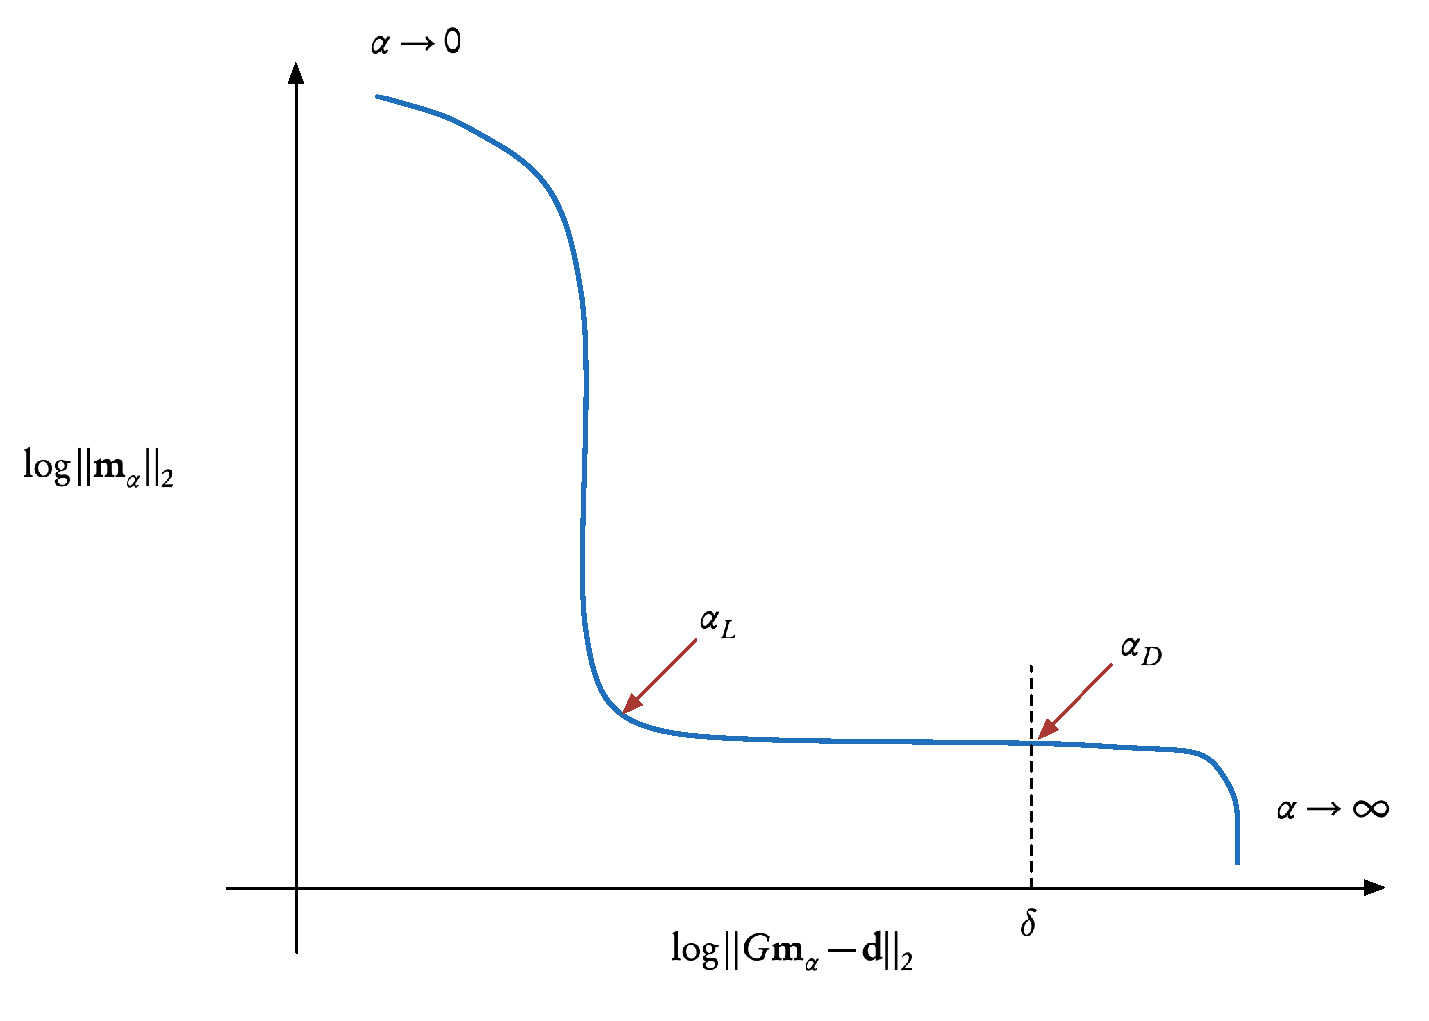
\includegraphics[width=0.8\textwidth]{graphics/L-curve}
\par\end{center}
\begin{itemize}
\item The\textbf{\textcolor{magenta}{{} L-curve criterion}} is an empirical
method for picking a value of $\alpha.$ 
\begin{itemize}
\item Since $e_{m}(\alpha)=\Vert\mathbf{m}\Vert_{2}$ is a strictly decreasing
function of $\alpha$ and $e_{d}(\alpha)=\Vert G\mathbf{m}-\mathbf{d}\Vert_{2}$
is a strictly increasing one, 
\item we plot $\log e_{m}$ against $\log e_{d}$ we will always obtain
an L-shaped curve that has an ``elbow'' at the optimal value of
$\alpha=\alpha_{L},$ or at least at a good approximation of this
optimal value\textemdash see Figure . 
\item This trade-off curve gives us a visual recipe for choosing the regularization
parameter, reminiscent of the bias-variance trade off
\item The range of values of $\alpha$ for which one should plot the curve
has to be determined by either trial-and-error, previous experience,
or a balancing of the two terms in the TR functional.
\end{itemize}
\item The\textbf{\textcolor{magenta}{{} discrepancy principle}}\emph{ }
\begin{itemize}
\item choose the value of $\alpha=\alpha_{D}$ such that the residual error
(first term) is equal to an \emph{a priori} bound, $\delta,$ that
we would like to attain. 
\item On the L-curve, this corresponds to the intersection with the vertical
line at this bound, as shown in Figure. 
\item A good approximation for the bound is to put $\delta=\sigma\sqrt{n},$
where $\sigma^{2}$ is the variance and $n$ the number of observations.\footnote{This is strictly valid under the hypothesis of i.i.d. Gaussian noise.}
This can be thought of as the noise level of the data. 
\item The discrepancy principle is also related to regularization by the
truncated singular value decomposition (TSVD), in which case the truncation
level implicitly defines the regularization parameter.
\end{itemize}
\item \textbf{\textcolor{magenta}{Cross-validation}}, as we explained in
ML Lectures, is a way of using the observations themselves to estimate
a parameter. 
\begin{itemize}
\item We then employ the classical approach of either LOOCV or $k$-fold
cross validation, and choose the value of $\alpha$ that minimizes
the RSS (Residual Sum of Squares) of the test sets. 
\item In order to reduce the computational cost, a generalized cross validation
(GCV) method can be used.
\end{itemize}
\end{itemize}

\foilhead{$\;$}

\vfill{}

\begin{center}
{\Large\textbf{\textcolor{blue}{DATA ASSIMILATION}}}{\Large\par}
\par\end{center}

\vfill{}


\foilhead{\textcolor{blue}{Definitions and notation}}
\begin{dinglist}{52}
\item \textcolor{magenta}{Analysis} is the process of approximating the
true state of a physical system at a given time
\item Analysis is based on:

\begin{dinglist}{52}
\item \textcolor{magenta}{observational }data,
\item a \textcolor{magenta}{model }of the physical system,
\item \textcolor{magenta}{background} information on initial and boundary
conditions.
\end{dinglist}
\item An analysis that combines time-distributed observations and a dynamic
model is called \textcolor{red}{data assimilation}.
\end{dinglist}

\foilhead{\textcolor{blue}{Standard notation}}
\begin{itemize}
\item A \textcolor{blue}{discrete model f}or the evolution of a physical
(atmospheric, oceanic, etc.) system from time $t_{k}$ to time $t_{k+1}$
is described by a dynamic, state equation
\begin{equation}
\mathbf{x}^{f}(t_{k+1})=M\left[\mathbf{x}^{f}(t_{k}),\right]\label{eq:state}
\end{equation}

\begin{itemize}
\item $\mathbf{x}$ is the model's state vector of dimension $n,$ 
\item $M$ is the corresponding dynamics operator (finite difference or
finite element discretization). 
\end{itemize}
\item The \textcolor{blue}{error covariance matrix} associated with $\mathbf{x}$
is given by $\mathbf{P}$ since the true state will differ from the
simulated state (\ref{eq:state}) by random or systematic errors.
\item \textcolor{blue}{Observations}, or measurements, at time $t_{k}$
are defined by
\[
\mathbf{y}_{k}^{\mathrm{o}}=H_{k}\left[\mathbf{x}^{t}(t_{k})\right]+\varepsilon_{k},
\]

\begin{itemize}
\item $H$ is an \textcolor{magenta}{observation operator}
\item $\varepsilon$ is a \textcolor{magenta}{white noise process} zero
mean and covariance matrix $\mathbf{R}$ (instrument errors and representation
errors due to the discretization)
\item observation vector $\mathbf{y}_{k}^{\mathrm{o}}=\mathbf{y}^{\mathrm{o}}(t_{k})$
has dimension $p_{k}$ (usually $p_{k}\ll n.$ )
\end{itemize}
\item Subscripts are used to denote the discrete time index, the corresponding
spatial indices or the vector with respect to which an error covariance
matrix is defined. 
\item Superscripts refer to the nature of the vectors/matrices in the data
assimilation process:

\begin{itemize}
\item ``a'' for \textcolor{magenta}{analysis}, 
\item ``b'' for \textcolor{magenta}{background} (or 'initial/first guess'), 
\item ``f'' for \textcolor{magenta}{forecast}, 
\item ``o'' for \textcolor{magenta}{observation} and 
\item ``t'' for the (unknown) \textcolor{magenta}{true} state.
\end{itemize}
\end{itemize}

\foilhead{\textcolor{blue}{Standard notation - continuous system}}
\begin{itemize}
\item Now let us introduce the continuous system. In fact, continuous time
simplifies both the notation and the theoretical analysis of the problem.
For a finite-dimensional system of ordinary differential equations,
the sate and observation equations become\index{data assimilation!continuous time}
\[
\dot{\mathbf{x}}^{\mathrm{f}}=\mathcal{M}(\xf,t)%\mathbf{\dot{\xf}}=\mathcal{M}(\xf,t)
\]
and 
\[
\yo(t)=\mathcal{H}(\xt,t)+\beps,
\]
where $\dot{\left(\,\right)}=\mathrm{d}/\mathrm{d}t,$ $\mathcal{M}$
and $\mathcal{H}$ are nonlinear operators in continuous time for
the model and the observation respectively.
\item This implies that $\x,$ $\y,$ and $\beps$ are also continuous-in-time
functions. 
\item For PDEs, where there is in addition a dependence on space, attention
must be paid to the function spaces, especially when performing variational
analysis. 
\item With a PDE model, the field (state) variable is commonly denoted by
$\boldsymbol{u}(\x,t),$ where $\x$ represents the space variables
(no longer the state variable as above!), and the model dynamics is
now a \textcolor{magenta}{nonlinear partial differential operator,}
\[
\mathcal{M}=\mathcal{M}\left[\partial_{\mathbf{x}}^{\alpha},\boldsymbol{u}(\mathbf{x},t),\mathbf{x},t\right]
\]
with $\partial_{\x}^{\alpha}$ denoting the partial derivatives with
respect to the space variables of order up to $\left|\alpha\right|\le m$
where $m$ is usually equal to two and in general varies between one
and four.
\end{itemize}

\foilhead{$\;$}

\vfill{}

\begin{center}
{\Large\textbf{\textcolor{blue}{CONCLUSIONS}}}{\Large\par}
\par\end{center}

\vfill{}


\foilhead{\textcolor{blue}{Introduction: conclusions}}

Data assimilation requires not only the observations and a background,
but also knowledge of:
\begin{dinglist}{52}
\item \textcolor{blue}{error statistics }(background, observation, model,
etc.) 
\item \textcolor{blue}{physics} (forecast model, model relating observed
to retrieved variables, etc.).
\end{dinglist}
The challenge of data assimilation is in \textcolor{magenta}{combining
}our stochastic knowledge with our physical knowledge.

\foilhead{Codes}

Various open-source repositories and codes are available for both
academic and operational data assimilation. 
\begin{enumerate}
\item DARC: \url{https://research.reading.ac.uk/met-darc/} from Reading,
UK. 
\item DAPPER: \url{https://github.com/nansencenter/DAPPER} from Nansen,
Norway. 
\item DART: \url{https://dart.ucar.edu/} from NCAR, US, specialized in
ensemble DA. 
\item OpenDA: \url{https://www.openda.org/}. 
\item Verdandi: \url{http://verdandi.sourceforge.net/} from INRIA, France. 
\item PyDA: \url{https://github.com/Shady-Ahmed/PyDA}, a Python implementation
for academic use. 
\item Filterpy: \url{https://github.com/rlabbe/filterpy}, dedicated to
KF variants. 
\item EnKF; \url{https://enkf.nersc.no/}, the original Ensemble KF from
Geir Evensen. 
\end{enumerate}

\foilhead{References}
\begin{enumerate}
\item K. Law, A. Stuart, K. Zygalakis. \emph{Data Assimilation. A Mathematical
Introduction}. Springer, 2015.
\item G. Evensen. \emph{Data assimilation, The Ensemble Kalman Filter},
2nd ed., Springer, 2009.
\item A. Tarantola. \emph{Inverse problem theory and methods for model parameter
estimation.} SIAM. 2005.
\item O. Talagrand. Assimilation of observations, an introduction. \emph{J.
Meteorological Soc. Japan}, \textbf{75}, 191\textendash 209, 1997.
\item F.X. Le Dimet, O. Talagrand. Variational algorithms for analysis and
assimilation of meteorological observations: theoretical aspects.
\emph{Tellus,} \textbf{38}(2), 97\textendash 110, 1986.
\item J.-L. Lions. Exact controllability, stabilization and perturbations
for distributed systems. \emph{SIAM Rev.}, \textbf{30}(1):1\textendash 68,
1988.
\item J. Nocedal, S.J. Wright. \emph{Numerical Optimization}. Springer,
2006.
\item F. Tr�ltzsch. \emph{Optimal Control of Partial Differential Equations}.
AMS, 2010.
\end{enumerate}

\end{document}
